%!TEX root = ../dokumentation.tex

\chapter{Materialien und Methoden} \label{ch:materialsAndMethods}

% TODO: Linguistische Begriffe (Semantik, Syntax, Pragmatik) erklären

% -   Politikapparat und Parteienlandschaft
% -   Erörterung, welche Medienplattformen und Nachrichtenquellen verwendet werden sollen
% -   Auswahl von Quellen und Sammeln von Daten
% -   NLP-Pipeline
% -   Machine Learning / Clustering

\section{Deutsche Politik in der 19. Legislaturperiode}

Dieser Abschnitt gibt ein Überblick über die politische Situation während der \num{19}. Wahlperiode des Deutschen Bundestages. Die politischen Themen und Aussagen spiegeln sich in den zu untersuchenden Texten wider. In \autoref{subsec:btw17} werden der Ausgang und die Folgen der Bundestagswahl \num{2017} beleuchtet und im Anschluss wird in \autoref{subsec:heterogenitätParteien} genauer auf die Parteienlandschaft und parteiinterne Unterschiede und Flügel eingegangen. Schließlich werden in \autoref{subsec:besondereEreignisse} besondere Ereignisse im Untersuchungszeitraum angeführt und in \autoref{subsec:themenschwerpunkte} diejenigen Themen erläutert, die während der Zeit den politischen Diskurs am stärksten geprägt haben.

\subsection{Bundestagswahl \num{2017}} \label{subsec:btw17}

Die Bundestagswahl \num{2017} fand am \num{24}. September \num{2017} statt. \autoref{fig:ergebnisBtw17} zeigt dazu die Aufteilung der Zweitstimmen nach Partei.

\begin{figure}[H]
    \centering
    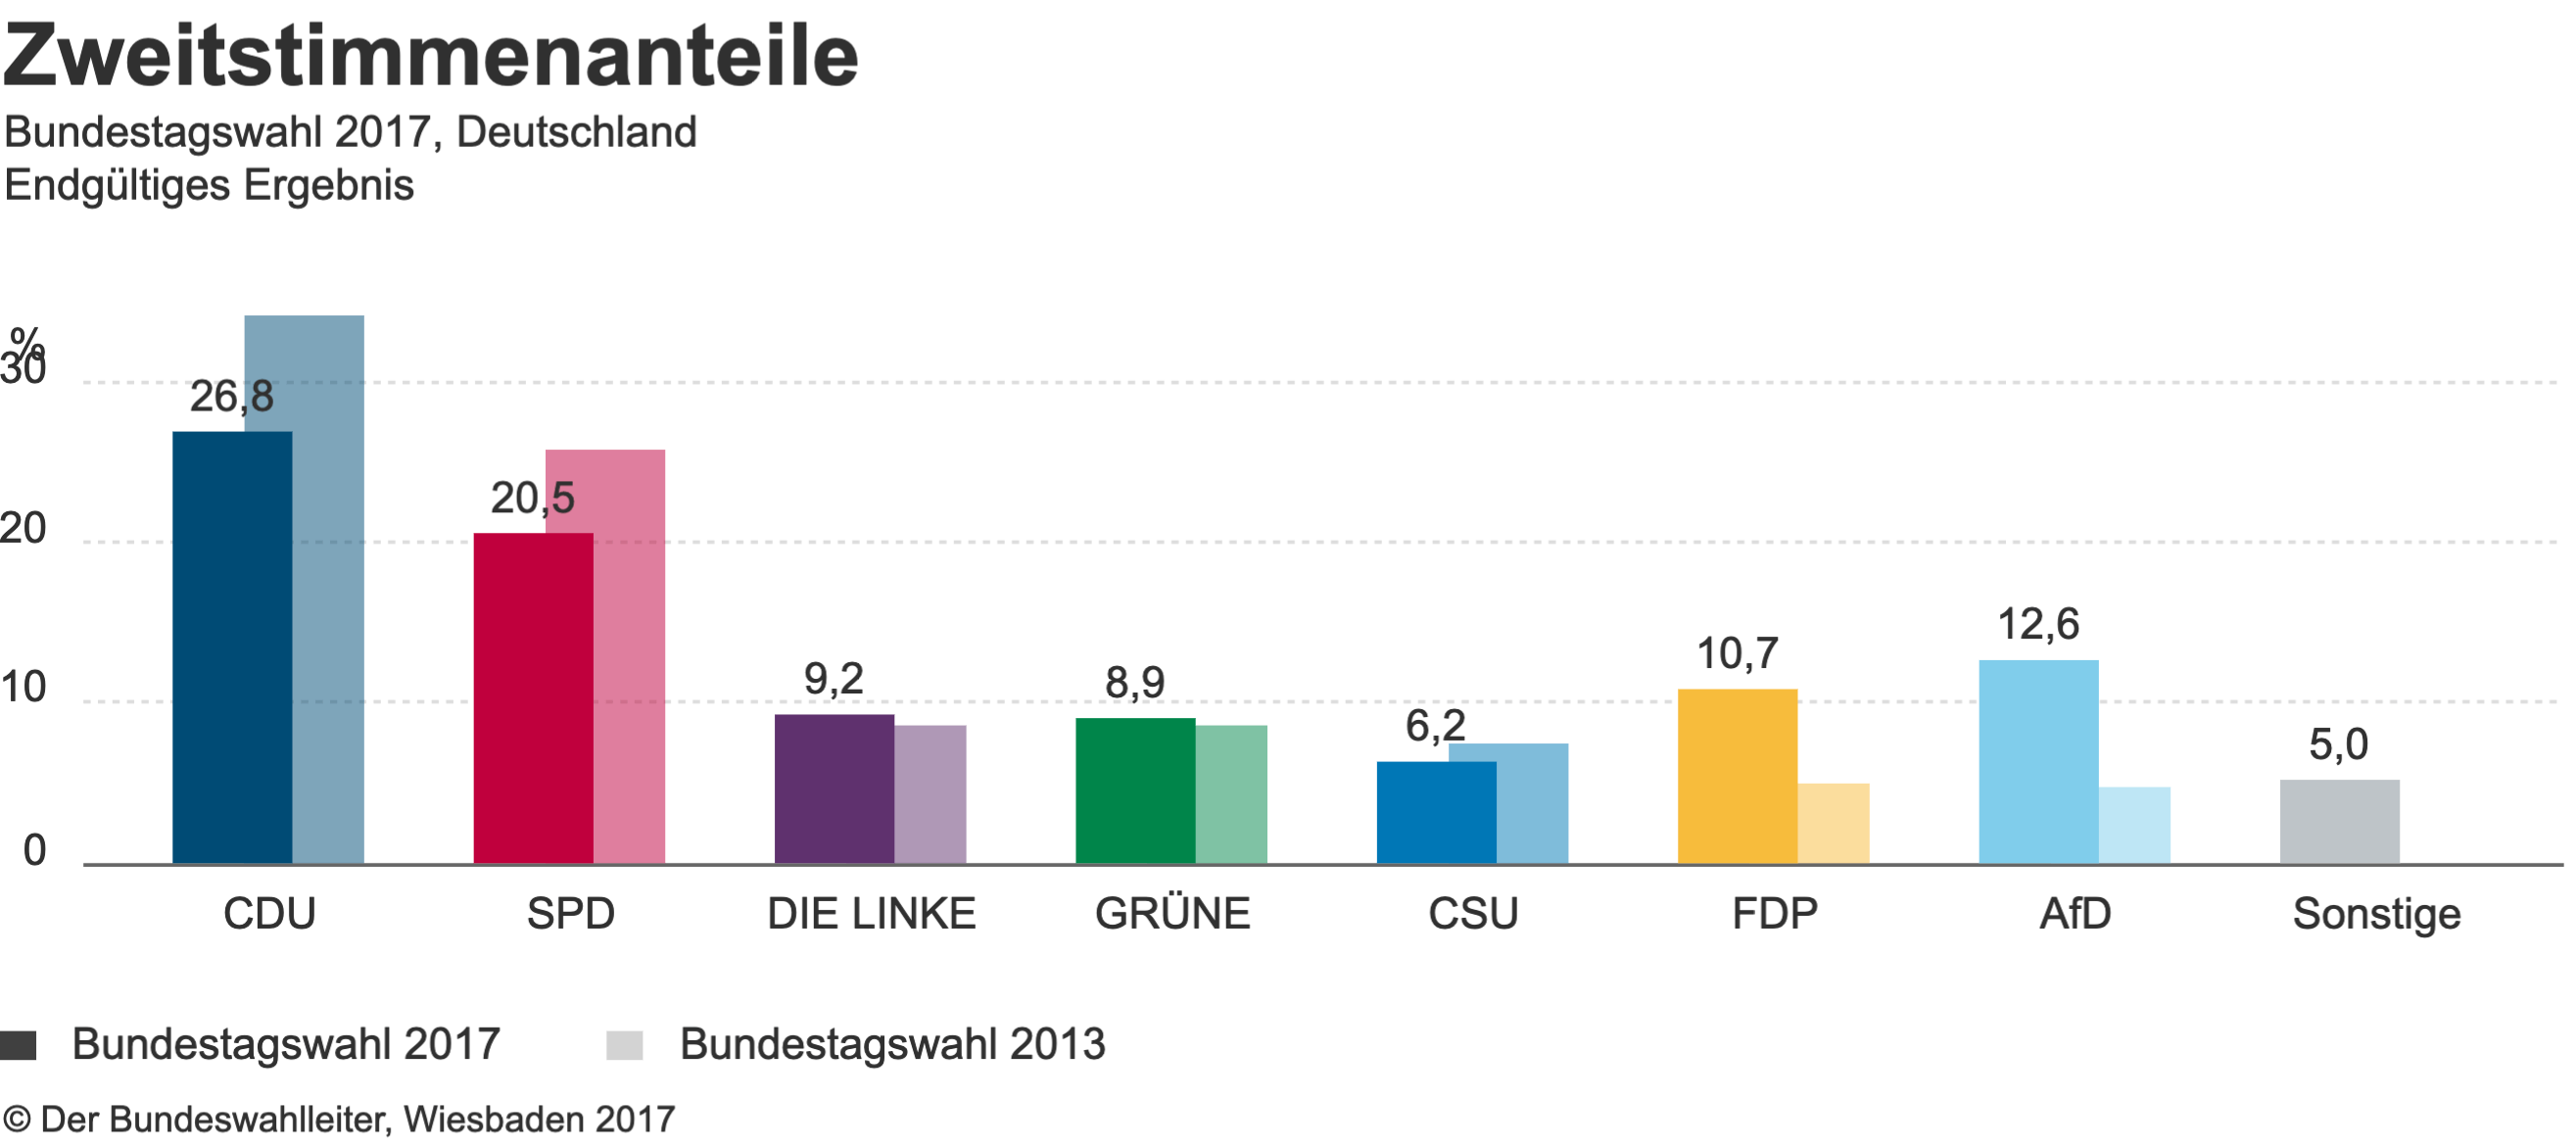
\includegraphics[width=0.9\textwidth]{data/images/ergebnisBtw17.png}
    \caption{Ergebnis der Bundestagswahl \num{2017} \autocite{noauthor_bundestagswahl_nodate}} \label{fig:ergebnisBtw17}
\end{figure}

Die \ac{CDU} erlitt zwar einen starken Verlust bezüglich der vorherigen Wahl, konnte sich aber dennoch mit \SI{26.8}{\percent} der Stimmen als stärkste Kraft durchsetzen. Gemeinsam kommen die \ac{CDU} und \acs{CSU} auf insgesamt \SI{32.9}{\percent}. Die \ac{SPD}, die ebenfalls im Vergleich zur Bundestagswahl \num{2013} an Stimmen verlor, kam auf \SI{20.5}{\percent}. Mit minimalen Steigerungen kamen die Linke auf \SI{9.2}{\percent} und die Grünen auf \SI{8.9}{\percent}. Sowohl die \ac{FDP} mit \SI{10.7}{\percent} als auch die \ac{AfD} mit \SI{12.6}{\percent} konnten ihre Anteile deutlich steigern. Während es die \ac{AfD} durch dieses Ergebnis zum ersten Mal in den Bundestag schaffte, konnte die \ac{FDP} nach dem Ausscheiden \num{2013} erneut in den Bundestag einziehen. Die übrigen Parteien kamen kumuliert auf \SI{5}{\percent} der Stimmen.

Laut \textcite{schmid_deutscher_2021} seien nach der Bundestagswahl \num{2017} zum ersten Mal sieben Parteien und sechs Fraktionen im Bundestag vertreten. Dies könne als Zeichen für die weiter abnehmende Bindungskraft der Volksparteien \ac{CDU}, \ac{CSU} und \ac{SPD} gesehen werden. Zudem seien besonders die starken Verluste von Union und \ac{SPD} hervorzuheben. Die \ac{SPD} verzeichnete mit der Bundestagswahl außerdem ihr schlechtestes Ergebnis seit \num{1949}.

Im Anschluss an die Wahl begonnen Sondierungsverhandlungen für eine mögliche \enquote{Jamaika-Koalition} zwischen Union, \ac{FDP} und Grünen. Nachdem diese seitens der \ac{FDP} abgebrochen wurden, bildete sich eine Große Koalition aus Union und \ac{SPD}. Damit gab es die längste Regierungsbildung in Deutschland aller Zeiten \parencite{schmid_deutscher_2021}.

\subsection{Heterogenität der Parteienlandschaft} \label{subsec:heterogenitätParteien}

Nach \textcite{niedermayer_entwicklung_2020} weist das deutsche Parteisystem einen Wandel, weg von den alten zwei Volksparteien (\ac{CDU} und \ac{SPD}), hinzu \enquote{einem pluralistischen System an der Grenze zum hochfragmentierten System} auf. Dabei sei besonders bei den Volksparteien ein schrittweiser Verlust der Zustimmung festzustellen, wohingegen sich die Grünen als zweitstärkste Kraft etabliert haben. Zudem habe sich auch die \ac{AfD} fest verankert. Bei der \ac{FDP} und der Linken sei wenig Dynamik zu erkennen.

\textcite{engler_wettbewerb_2022} heben hervor, dass bei vielen Themen die Oppositionsparteien divergente Meinungen entgegen der Regierung und auch untereinander vertreten. Während die Grünen und Linke für konsequentere Klimamaßnahmen plädieren, positioniert sich die \ac{AfD} entgegengesetzt. In der Debatte um \ac{COVID-19}-Maßnahmen ergebe sich ein ähnliches Bild, in der sich auch die \ac{FDP} kritisch gegen einige Maßnahmen positioniert habe.

Die politischen Parteien in Deutschland grundlegend in zwei Lager eingeteilt werden: Ein \enquote{links-liberales} bestehend aus \ac{SPD}, Grünen und Linken, sowie ein \enquote{rechts-konservatives} oder \enquote{bürgerliches} bestehend aus der Union und \ac{AfD} \autocite{thomeczek_politische_2019}. Der \ac{FDP} wird als gesellschaftspolitisch liberale, aber wirtschaftspolitisch rechte Partei eine Sonderrolle zugeschrieben. Zudem beobachten \textcite{thomeczek_politische_2019}, dass die Parteien eine unterschiedliche interne Kohärenz aufweisen. Die beiden Volksparteien, \ac{SPD} und \ac{CDU}, weisen dabei durchschnittlich weniger hohe Agreement-Index-Werte -- ein Maßstab, wie stark die Positionen der Mitglieder übereinstimmen -- auf als die anderen Parteien.

Die Verteilung der Positionen innerhalb einer Partei betrachtet auch \textcite{saltzer_bundestagswahl_2022}. \autoref{fig:positionierungAusgewaehlterKanidaten} zeigt die Verortung von Kandidaten für die Bundestagswahl \num{2021} nach Partei. Die x-Achse stellt dabei die Position in der politischen Links-Rechts-Skala und die y-Achse die Zustimmung zu Regierung beziehungsweise Opposition.

\begin{figure}[H]
    \centering
    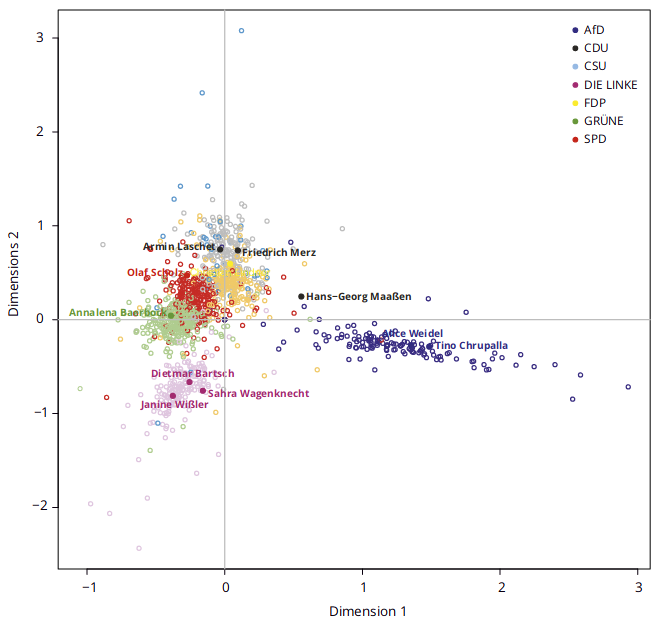
\includegraphics[width=0.5\textwidth]{data/images/positionierung_ausgewaehlter_kandidaten.png}
    \caption[Positionierung ausgewählter Kandidaten \autocite{saltzer_bundestagswahl_2022}]{Positionierung ausgewählter Kandidaten innerhalb eines zweidimensionalen politischen Raums \autocite{saltzer_bundestagswahl_2022}} \label{fig:positionierungAusgewaehlterKanidaten}
\end{figure}

Aus der Grafik geht hervor, dass besonders Parteien an den Rändern des politischen Spektrums -- Linke und \ac{AfD} -- sich von den restlichen Parteien visuell abgrenzen. Die restlichen Parteien verteilen sich rund um den Ursprung des Koordinatensystems herum und überschneiden sich dabei auch.

Kandidaten der Union und \ac{FDP} liegen im Schnitt in der Mitte der Links-Rechts-Skala. Dabei liegt die Regierungs-Zustimmung der Union höher. Im Vergleich zur \ac{FDP} ist die \ac{SPD} weiter links positioniert. Die Kandidaten der Grünen sind noch weiter links eingezeichnet und neutral auf der y-Achse. Die Linke befinden sich ähnlich weit links wie die Grünen, sind aber deutlich eher der Opposition zugeneigt. Die \ac{AfD} ist die einzige Partei, die nach der gegebenen Darstellung rechts der Mitte aufzufinden ist und dabei eher der Opposition nahesteht.

Auffällig ist, dass die Verteilung der \ac{AfD}-Kandidaten auf der Links-Rechts-Skala deutlich stärker verstreut ist im Vergleich zu den anderen Parteien. Eine mögliche Begründung ist der Protest gegen die herkömmlichen Parteien. Daraus ergibt sich eine niedrigere interne Einigkeit zu politischen Themen und eine stärkere Streuung der Meinungen.

\subsection{Besondere Ereignisse im Untersuchungszeitraum} \label{subsec:besondereEreignisse}

\textcite{schmid_deutscher_2021} gibt wichtige öffentlichkeitswirksame Ereignisse während der \num{19}. Wahlperiode des deutschen Bundestages wieder. Darunter fällt zunächst die \ac{COVID-19}-Pandemie, der Auswirkungen und der Umgang mit diesen nach den ersten Ansteckungsfällen Anfang 2020 zu einem zentralen Thema in Politik und Gesellschaft wurden. Im Juli 2021 kam es in Teilen von Nordrhein-Westfalen und Rheinland-Pfalz zu einer schweren Flutkatastrophe. Kurz vor Ende der Legislaturperiode wurde zudem der Einsatz der Bundeswehr in Afghanistan beendet, nachdem eine Machtübernahme der Taliban erfolgt war.

Neben der Bundestagswahl \num{2017} fand am 29. Mai 2019 die Wahl des Europäischen Parlaments statt. Zudem wurden in der Periode \num{13} Landtagswahlen ausgerichtet.

\subsection{Themenschwerpunkte} \label{subsec:themenschwerpunkte}

\textcite{engler_wettbewerb_2022} untersuchen die Themenschwerpunkte in politischen Debatten während der \num{19}. Wahlperiode. Anhand von Umfragen der Forschungsgruppe Wahlen ergibt sich folgender Verlauf. Dieser zeigt die Zu- und Abnahme an Relevanz der Themen, die in der Zeitperiode Relevanz hatten.

\begin{figure}[H]
    \centering
    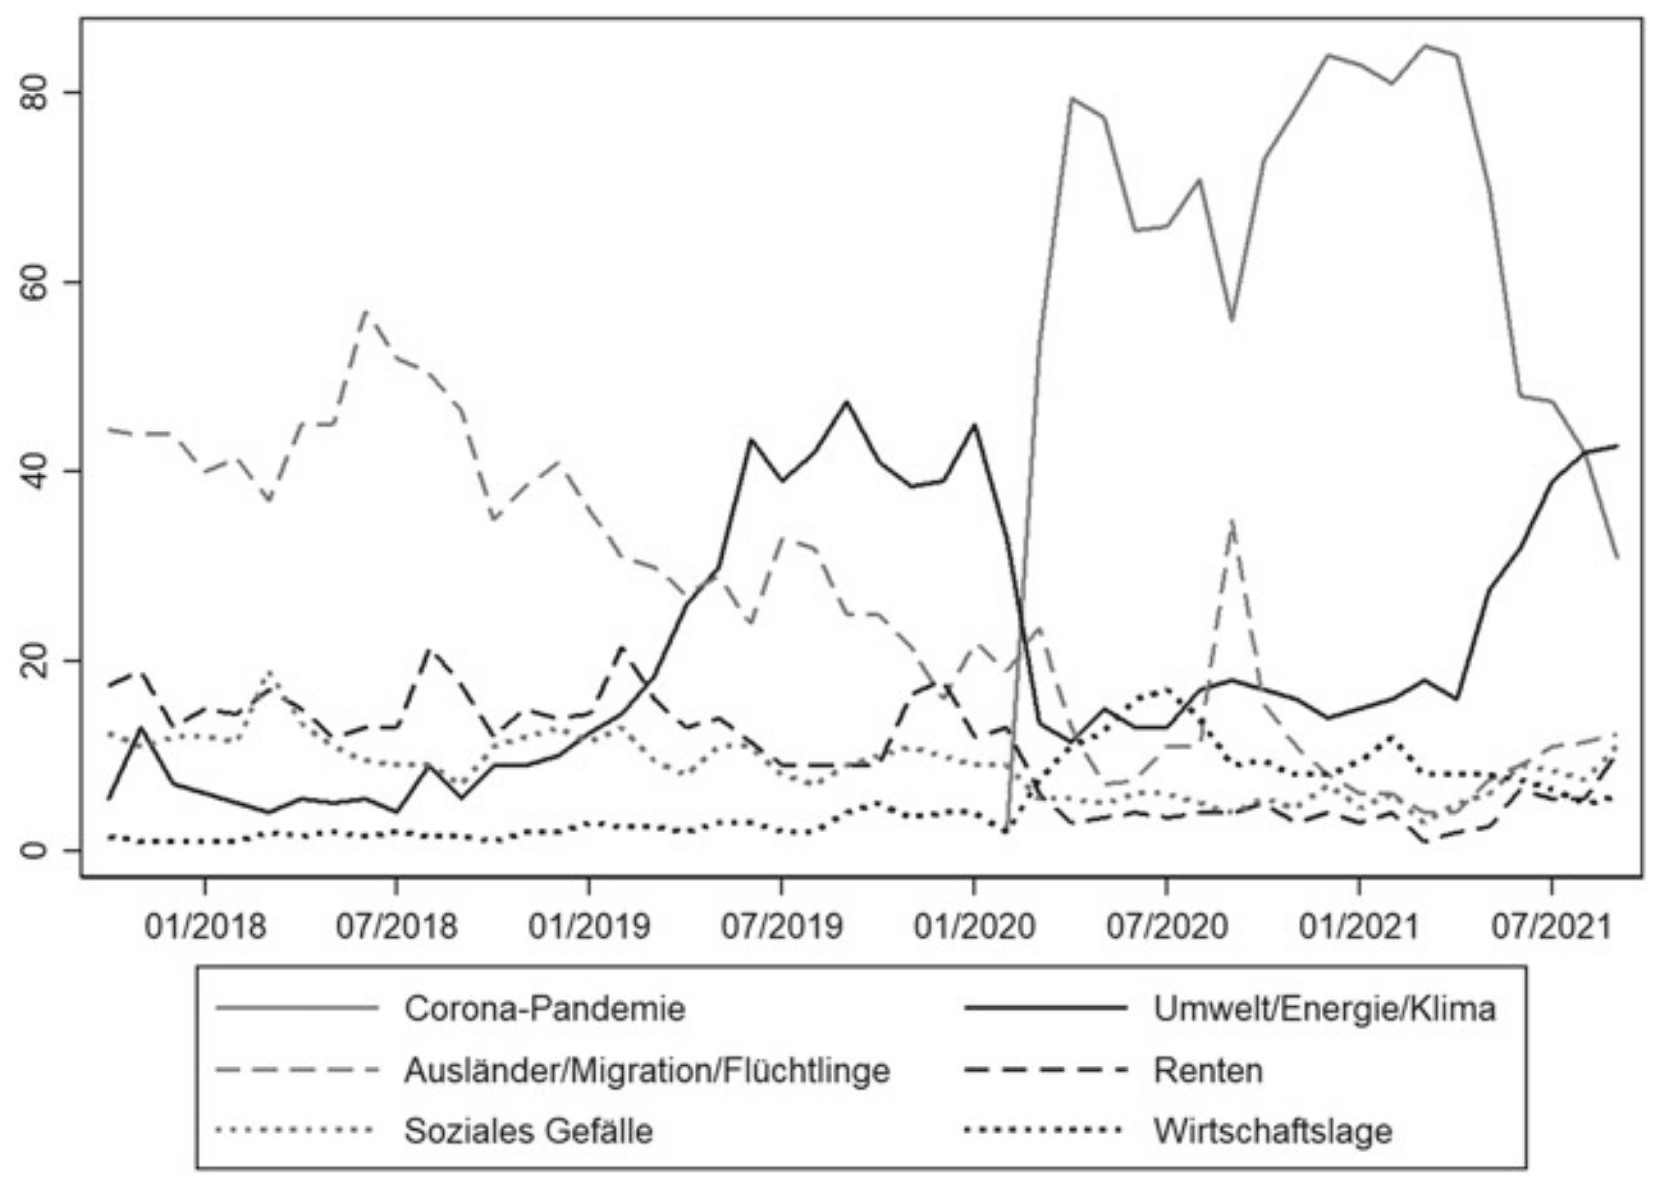
\includegraphics[width=0.8\textwidth]{data/images/themenkonjunktur.png}
    \caption{Verlauf der wichtigsten politischen Themen während der 19. Wahlperiode \autocite{engler_wettbewerb_2022, forschungsgruppe_wahlen_forschungsgruppe_nodate}} \label{fig:themenkonjunktur}
\end{figure}

Zu Beginn der Legislaturperiode war das Thema der Migrationspolitik am wichtigsten. Die Relevanz hat jedoch stetig abgenommen, bis das Thema ab \num{2020} untergeordnet war. Der Themenbereich Umwelt, Energie und Klima wurde ab \num{2019} immer wichtiger und war zeitweise das Thema mit der meisten Relevanz. Nach der Flutkatastrophe \num{2021} wurde diesem Bereich wieder vermehrt Bedeutung zugesprochen. Nach dem Ausbruch der Pandemie war diese schlagartig das mit Abstand dominierende Thema, bis sich die Lage \num{2021} wieder beruhigte. Während des gesamten Zeitraums rückten wirtschafts- und sozialpolitische Themen in den Hintergrund.

Nach \textcite{niedermayer_entwicklung_2020} waren im Betrachtungszeitraum vorwiegend die Flüchtlingskrise sowie das Thema Klimawandel und Energiewende von Bedeutung. Die Dominanz der Klimathematik zeigt sich an Ereignissen wie dem Dieselskandal, der Hitzewelle im Sommer \num{2018} sowie der Popularität der Protestbewegung \enquote{Fridays for Future}.

\section{Repräsentationsformen von Text} \label{sec:representationForms}

% TODO: Either describe specific models or the underlying architecture (e.g. fasttext or n-gram method)

Um Analysen und \ac{ML} auf Text anwenden zu können, ist es notwendig diesen Vektoren umzuwandeln, die durch Maschinen interpretierbar sind. Abhängig von der Methodik wird dabei die Integrität der syntaktischen und semantischen Beziehungen beeinflusst \autocite{kowsari_text_2019, jurafsky_speech_2023}.

Methoden wie \ac{BoW} und \ac{TF-IDF} generieren unkomprimierte Vektoren und skalieren linear mit der Anzahl an einzigartigen Wörtern. Diese Verfahren können jedoch nicht den Kontext innerhalb eines Satzes abbilden. Ein alternativer Ansatz ist die Repräsentation mittels kontextabhängigen Verfahren. Mittels neuronalen Netzen können Zusammenhänge innerhalb eines Satzes erkannt werden. Beispielhafte Implementierungen sind \ac{LSTM}-Netzwerke, als auch \ac{ELMo}.

% TODO: Transformer Modelle

Worteinbettungen (engl. Word Embeddings) repräsentieren eine zentrale Rolle, bei der Analyse und dem Training von \ac{NLP} Modellen. Diese bilden einzigartige Wörter mittels mehrdimensionalen Vektoren\footnote{Häufig bestehen Word Embeddings aus \num{300} Dimensionen} ab. Abhängig vom Verfahren sind die resultierenden Vektoren komprimiert oder unkomprimiert. Worteinbettungen ermöglichen es, Wörter mit einer ähnlichen Bedeutung im mehrdimensionalen Raum nah beieinander zu gruppieren.

Die unterschiedlichen Verfahren können auf Wort-, Satz- oder Dokumentebene angewendet werden.

\subsection{Kontextunabhängig}

\ac{BoW} und \ac{TF-IDF} extrahieren Informationen über die Häufigkeit einzelner Wörter. Beide Verfahren geben somit Aufschluss über den Inhalt und Themen einzelner Texte. Jedoch ermöglichen die Verfahren nicht, den genauen Kontext, Grammatik und Satzbau zu analysieren. 

% TODO: Beide Verfahren zu einer großen Anzahl an Features (unkompromiert)

\subsubsection*{N-Gram}

N-Grams sind die Grundlage für Verfahren wie \ac{BoW} und \ft. Bei dieser Methode werden Zeichen (Wortebene) oder Wörter (Satzebene) in Fragmente mit der Länge \texttt{n} unterteilt \autocite[5]{kowsari_text_2019}. Die Reihenfolge der Elemente bleibt dabei unverändert.

\subsubsection*{\acl{BoW}} 

\ac{BoW} ist eine simple Repräsentationsform, die lediglich die Häufigkeit von einzigartigen Wörtern berechnet \autocite[6]{kowsari_text_2019}. Im ersten Schritt des Verfahrens, wird ein Satz oder Dokument in eine Menge an 1-Grams (einzelne Wörter) transformiert. Anschließend wird die Liste auf die einzigartigen Wörter reduziert und gezählt, wie häufig die einzigartigen Wörter (engl. Features) auftreten. Die daraus entstehende Tabelle wird auch \ac{BoF} genannt.

Um zu demonstrieren, wie \ac{BoW} funktioniert, nennt \textcite[6]{kowsari_text_2019} folgendes Beispiel: \enquote{As the home to UVA’s recognized undergraduate and graduate degree programs in systems engineering. In the UVA Department of Systems and Information Engineering, our students are exposed to a wide range of range.} Aus dem Text resultiert die folgende \ac{BoF} Tablle: \enquote{\{1,1,1,3,2,1,2,1,2,3,1,1,1,2,1,1,1,1,1,1\}}.

Da \ac{BoW} ein Verfahren ist, welche die Reihenfolge von Wörtern nicht berücksichtigt, kann es zum Beispiel nicht zwischen \textit{\enquote{Das ist gut}} und \textit{\enquote{Ist das gut}} unterscheiden \autocite[6]{kowsari_text_2019}.

\subsubsection*{\acl{TF-IDF}}

Neben der reinen Häufigkeit berücksichtigt \ac{TF-IDF} außerdem die Häufigkeit eines Wortes für eine Sammlung an Dokumenten \autocite[7]{kowsari_text_2019}. Damit ist es möglich Wörter, aus Wortgruppen wie Artikeln, Präpositionen, Konjunktionen von relevanten Wörtern (meist Adjektive, Verben und Nomen) zu trennen.

\[\mathrm{tfidf}(t,d,D) = \frac{f_{t,d}}{{\sum_{t' \in d}{f_{t',d}}}} \cdot \log \frac{N}{|\{d \in D: t \in d\}|}\]

Dafür wird zunächst die relative oder absolute Häufigkeit eines Wortes innerhalb eines Dokumentes berechnet. Außerdem wird die Häufigkeit in anderen Dokumenten berechnet. Der sich daraus ergebene Wert gibt Auskunft darüber, ob es sich um ein generell häufiges Wort oder nicht handelt.

% \subsubsection*{CBOW und Skip-Gram}

% \begin{figure}[H]
%     \centering
%     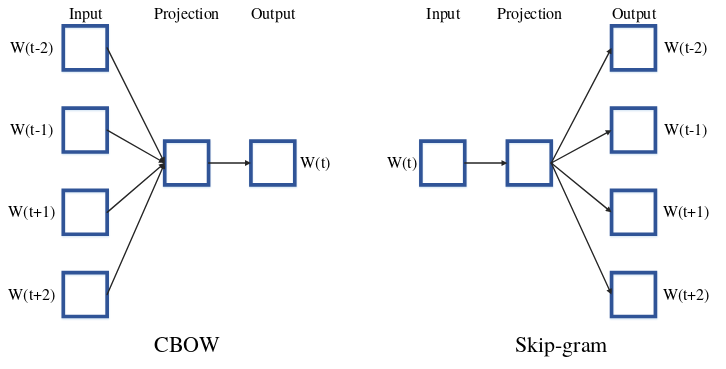
\includegraphics[width=0.6\textwidth]{data/images/materials_and_methods/cbow_skip_gram.png}
%     \caption{\autocite[8]{kowsari_text_2019}}
%     \label{fig:cbow_skip_gram}
% \end{figure}

% TODO: Entfernen -> Für weitere Informationen verweisen wir auf ...

\subsubsection*{Word2Vec, GloVe}

% TODO: Beispiel -> König - Mann + Frau = Königin
% TODO: Problem -> Bank liefert Vektor zwischen Parkbank und Geldinstitut
% TODO: Möglicher Bias -> Arzt - Mann + Frau = Krankenschwester
% TODO: Nur nahestehende Stymbolde werden als Kontext interpretiert

CBOW und Skip-Gram -> siehe ...

\subsubsection*{fastText}

Anstelle von ganzen Wörtern, verwendet \ft zum Trainieren und Klassifizieren n-grams bestehend aus \textit{n} Zeichen \autocite{kowsari_text_2019, joulin_fasttextzip_2016}. Ein Beispiel ist das Wort \textit{Tischtennis}, welches mit \(n = 3\) in \textit{<Ti,Tis,isc,sch,cht,hte,ten,enn,nni,nis,is>} zerlegt wird. Wörter, die in ähnliche n-grams zerlegt werden können, resultieren in Vektoren, welche nah im Vektorraum beieinanderliegen. Die Optimierung während des Trainings und Klassifikation erfolgt mittels der Softmax-Funktion. Zusätzlich wird bag-of-n-grams genutzt, um Zusammenhänge in einem Text zu erkennen \autocite[2]{joulin_bag_2016}. Aufgrund der n-gram Methodik und der niedrigen Komplexität von \(O(h \log_{2}(k))\) des Optimierungs- und Klassifikationsverfahren, eignet sich \ft für die Klassifikation von großen Mengen an Text \autocite[2\psqq]{joulin_bag_2016}.

Im Vergleich zu Word2Vec lassen sich mittels \ft auch Wörter klassifizieren, die nicht Teil des Trainings waren. Dies ist besonders bei komplexen Sprachen, welche zusammengesetzte Wörter verwendet\footnote{Beispiel: Tischtennis lautet im Englischem \textit{table tennis}.}, hilfreich.

Skip-Gram -> siehe ...

\subsection{Kontextabhängig}

Um syntaktische und semantische Beziehungen zu erkennen, ist es notwendig, nicht nur den Satzbau, sondern auch die Bedeutung einzelner Wörter schon mittels der Methodik zur Transformation zu berücksichtigen. Kontextabhängige Worteinbettungen verwenden meist einen Speicher an vorherigen Wörtern, um den Kontext zu darauffolgenden Wörtern herzustellen.

% \subsubsection*{LSTM}

% Lorem Ipsum

% \subsubsection*{ELMo}

% Lorem Ipsum

\subsection{Transformer}

% TODO: Add and describe models used for modeling

\subsubsection*{BERT}

% Lorem Ipsum

\section{Sentimentanalyse} \label{sec:sentimentanalysis}

Eine Limitation von herkömmlichen \ac{ML} Modellen ist die Klassifikation von Polysemie \autocite[48\psq]{kowsari_text_2019}. Ein Ansatz, um diese Limitation zu mindern, ist es, den Sentiment eines Textes zu berechnen. Ziel dieser Technik ist es nicht nur festzustellen, ob sich beispielsweise ein Politiker zu einem gewissen Thema äußert oder nicht, sondern ebenfalls, ob seine Äußerungen positiv, neutral oder negativ sind.

Herkömmliche Methoden zur Bestimmung des Sentiments von deutschen Texten sind \textcite[1627\psq]{guhr_training_2020} zufolge Sentiment-Wörterbücher und Machine Learning Modellen wie \ac{SVM}, \ac{CNN} und \ac{Bi-LSTM}. Alle genannten Methoden erreichen einen $F_1$ Score von \numrange{46.5}{74.9}

Die Arbeit von \textcite{guhr_training_2020} zeigt, wie sich Texte anhand ihres Sentiments -- positiv, neutral, oder negativ -- durch \ac{BERT} klassifizieren lassen. Für das Training nutzen die Autoren acht unterschiedliche Datensätze, die insgesamt \num{5.3} Millionen Einträge umfassen. Neben einem \ac{BERT} Modell wurde ebenfalls ein Modell mittels \ft trainiert. Dieses erreicht jedoch einen leicht schlechteren $F_1$ Score\footnote{Mit dem unbalancierten Datensatz erreicht \ac{BERT} einen $F_1$ Score von \num{97.44} und \ft \num{95.73}. Bei dem balanciertem Datensatz erreicht \ac{BERT} einen $F_1$ Score von \num{96.36} und \ft \num{94.05}.} als das \ac{BERT} Modell \autocite[\psq 1630]{guhr_training_2020}.

Auffällig ist, dass das Modell einen signifikant schlechteren $F_1$ Score erreichen, wenn der Datensatz Tweets oder andere Social Media Posts inkludiert. Dies zeigt sich bei den Datensätzen PlotTS, SB10k und GermEval-2017. Bei der Klassifikation dieser erreicht das Modell lediglich einen $F_1$ Score von \numrange{0.6423}{0.7885} \autocite[1631]{guhr_training_2020}.

\section{Zusammenfassung}

Im ersten Abschnitt des Kapitels wird die politische Situation in Deutschland zur Zeit der \num{19}. Legislaturperiode skizziert. Die Volksparteien \ac{CDU}/\ac{CSU} und \ac{SPD} haben bei der Bundestagswahl \num{2017} Verluste hinnehmen müssen, bilden jedoch eine Große Koalition. Die Grünen und die \ac{AfD} erleben einen Aufschwung und sorgen so dafür, dass das Parteiensystem diverser wird. Im Untersuchungszeitraum bestimmten hauptsächlich die Themenbereiche Migration, Klimaschutz und Pandemie den Diskurs.

Der zweite Abschnitt des Kapitels umreißt die Basismethoden zur Analyse und Klassifizierung von Texten. \ac{BoW} und \ac{TF-IDF} sind die beiden einfachsten Methoden, die lediglich die Häufigkeit einzigartiger Wörter betrachten. \ac{BoW} betrachtet dabei ein einzelnes Dokument, während \ac{TF-IDF} auch die Häufigkeit über mehrere Dokumente hinweg berücksichtigt. Im Gegensatz zu diesen beiden unkomprimierten Verfahren nutzen Word2Vec, GloVe und \ft komprimierte Vektoren, die Wörter oder Zeichen basierend auf ihrem Kontext einem Vektor im Vektorraum zuordnen.

Für die Analyse mittels deskriptiver Statistik in \autoref{ch:crispDm_1} wird ein Modell zur Bestimmung der Stimmung eines Textes betrachtet. Dieses Modell liefert Aufschluss darüber, ob ein Text positiv, negativ oder neutral klingt.
